\documentclass{article}
\usepackage{graphicx}
\graphicspath{ {Images/} }


\author{Pseudo-Ku}
\title{Java Sudoku Solver using Backtracking}
\date{07 October 2020}

\begin{document}
    \begin{titlepage}
        \maketitle{}
    \end{titlepage}
    
    \tableofcontents

    % Aims
    \pagebreak 
    \section{Aims}
    The main aim of this lab report is to review the performance of our group’s implementation of the Backtracking Algorithm on solving sudoku puzzles with varying amounts of zero spaces in the initial puzzle. Conversely, one could also interpret it as reviewing the algorithm’s performance on solving sudoku puzzles with varying amounts of filled spaces or clues in the initial puzzle. In this report we hypothesize that the more open spaces (or the fewer number of clues) there are in the initial sudoku puzzle, then the more computation will be required to solve such a puzzle. 
    It is thus our goal to verify our theoretical assumptions (which will be expanded upon in subsequent sections) of the algorithm’s performance with the empirical evidence we obtain from running our program on many different sudoku puzzles. Simply put, we want to check that the algorithm has the best, worst and average case complexities that we believe it to have theoretically. If this is not the case, then it is also our goal to determine why it is not.

    % Summary of Theory
    % \pagebreak 
    \section{Summary of Theory}

    % Experimental Methodology
    \pagebreak 
    \section{Experimental Methodology}
    As stated in our aims, our initial assumption is that more open spaces (or fewer clues) in the initial sudoku puzzle will result in more computation needed in order to find the unique solution of a given puzzle. We have utilized 3 metrics to measure the performance of the algorithm, namely number of comparisons, number of changes, and the amount of time taken to return a unique solution to a given puzzle. Please see below discussions on our chosen metrics:

    \subsection{Number of comparisons}
    This metric measures the number of times the program compares the current value of the puzzle it is on with the rest of the incomplete puzzle. At each iteration, the program checks that the current value does not break the puzzle (ie: it checks to see that the current value of the puzzle is not repeated within that value’s row, column or sub-grid. It is our assumption that puzzles with more empty spaces will need more comparisons than puzzles with less empty spaces. \cite{{inproceedings}}

    \subsection{Number of changes}
    This metric measures the number of times the program changes a value it has just compared to a value that will not break the board (since it found that the value at the position is currently on has broken the board). It also measures the number of times the program changes an empty space to a filled space (a space with any positive integer less than 10).
    Again, our group assumes that the program will make more changes to puzzles with more empty spaces than it will to puzzles with less empty spaces. 

    \subsection{Run Time}   
    This metric measures the length of time (in milliseconds) it takes for the program to output a unique solution to a given puzzle. It is our assumption that puzzles with more empty spaces will take much longer to complete than puzzles with less empty spaces. 

    *Add in* : 2 implementations – one random and one done linearly (adding in white spaces)
    - also add in that we initially tried doing difficulty, but results were not as comprehensible as the ones we get with the three chosen metrics. And also graphs look the same for difficulty (ie: the hardest easy graphs will look similar to the easiest medium graphs)
    - also add in that it’s difficult to define difficulty, because it’s not only number of clues that matter, but also the position of those clues that will matter as well.

    
    % Presentation of results
    \pagebreak 
    \section{Presentation of results}
    \begin{figure}[h]
        \centering
        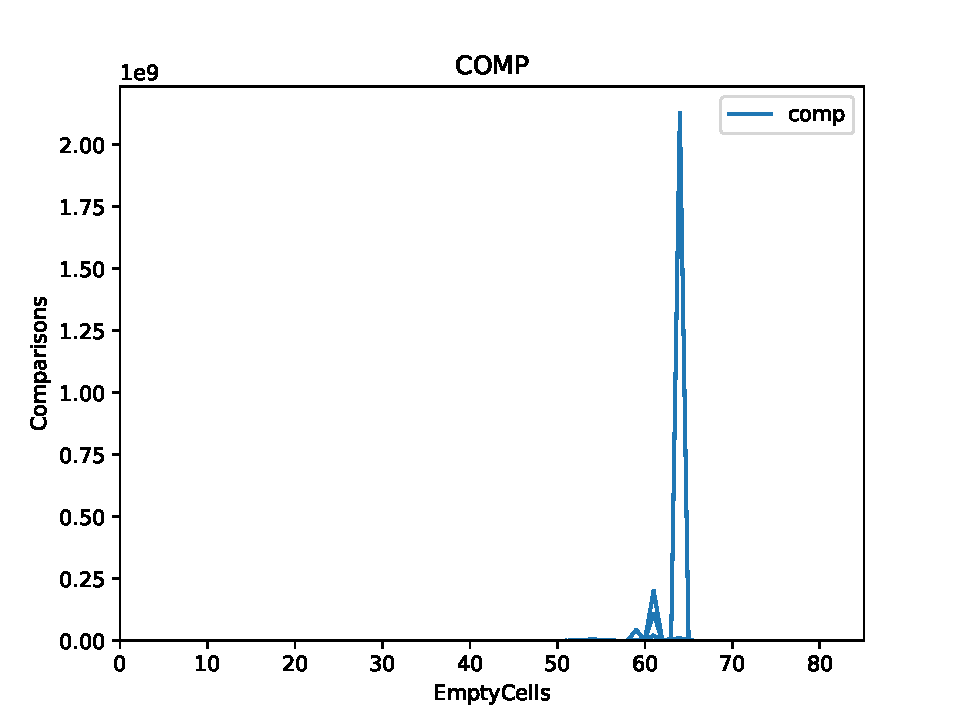
\includegraphics[width=1\textwidth]{COMP.pdf}
        \caption{Comparisons Plot}
    \end{figure}
        

    % Interpretation of results
    % \pagebreak 
    \section{Interpretation of results}

    % Theory relationship
    % \pagebreak 
    \section{Theory relationship}

    % Conclusion
    % \pagebreak 
    \section{Conclusion}

    % References
    \pagebreak
    \section{References}
    \bibliographystyle{plain}
    \bibliography{file.bib}

    % Acknowledgements
    % \pagebreak 
    \section{Acknowledgements}
\end{document}